% 图 1.8 黎曼球面：自旋 1/2 粒子自旋态的几何表示
\documentclass[tikz,border=5pt]{standalone}
\usetikzlibrary{arrows.meta}
\usepackage{amsmath}
\usepackage{bm}
\usepackage{fontspec}
\setmainfont{Times New Roman}
\begin{document}
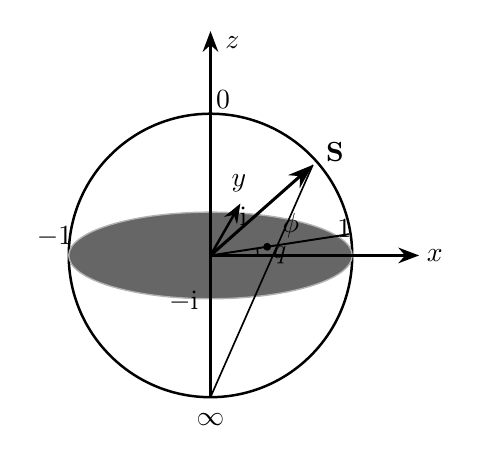
\begin{tikzpicture}[line width=0.9pt,>=Stealth]
% 球体轮廓
\draw (0,0) circle (1.8);
% 赤道面（阴影圆盘）
\fill[black!60] (0,0) ellipse (1.8 and 0.55);
\draw[line width=0.5pt,black!30] (0,0) ellipse (1.8 and 0.55);
% z 轴
\draw[->,line width=1.0pt] (0,-1.8) -- (0,2.85);
\node at (0.28,2.7) {$z$};
\node at (0.16,1.98) {$0$};
\node at (0,-2.08) {$\infty$};
% x 轴
\draw[->,line width=1.0pt] (0,0) -- (2.65,0);
\node at (2.85,0) {$x$};
\node at (1.7,0.34) {$1$};
\node at (-1.98,0.24) {$-1$};
% y 轴（指向观察者）
\draw[->,line width=0.9pt] (0,0) -- (0.38,0.66);
\node at (0.36,0.92) {$y$};
% 赤道面上的记号 i 与 -i（在 y 轴及其反向延长线上）
\node at (0.42,0.5) {$\mathrm{i}$};
\node at (-0.34,-0.59) {$-\mathrm{i}$};
% S 的投影线与方位角 phi
\draw[line width=0.7pt] (0,0) -- (1.76,0.27);
\draw[line width=0.6pt] (0.6,0) arc[start angle=0,end angle=9,radius=0.6];
\node at (1.02,0.38) {$\phi$};
% 连线与赤道面的交点 q
\fill (0.72,0.11) circle (0.05);
\node at (0.88,0.0) {$q$};
% 自旋矢量 S 与到南极的射线
\draw[line width=1.1pt,-{Stealth[length=3.2mm,width=2.2mm]}] (0,0) -- (1.3,1.15);
\node at (1.58,1.32) {$\mathbf{S}$};
\draw[line width=0.6pt] (1.3,1.15) -- (0,-1.8);
\end{tikzpicture}
\end{document}
